%!TEX program = xelatex
\documentclass[11pt]{beamer}

\usepackage{amsfonts}
\usepackage{amsmath}
\usepackage{blindtext}
\usepackage{enumitem}
\usepackage{fancyvrb}
\usepackage{tikz}

\usetheme{SaoPaulo}

\title{Numerical Python}
\subtitle{randomness}
\author{CS101 Lecture \#18}
\date{2016-10-31}

% Hallowe'en image?

\setcounter{showSlideNumbers}{1}

\newcommand{\correctstar}{\textcolor{red}{$\star$}}

\begin{document}
  \setcounter{showProgressBar}{0}
  \setcounter{showSlideNumbers}{0}

%%%%%%%%%%%%%%%%%%%%%%%%%%%%%%%%%%%%%%%%%%%%%%%%%%%%%%%%%%%%%%%%%%%%%%%%%%%%%%%%
\frame{\titlepage}

%%%%%%%%%%%%%%%%%%%%%%%%%%%%%%%%%%%%%%%%%%%%%%%%%%%%%%%%%%%%%%%%%%%%%%%%%%%%%%%%
\setcounter{framenumber}{0}
\setcounter{showProgressBar}{1}
\setcounter{showSlideNumbers}{1}

%%%%%%%%%%%%%%%%%%%%%%%%%%%%%%%%%%%%%%%%%%%%%%%%%%%%%%%%%%%%%%%%%%%%%%%%%%%%%%%%
\section{Administrivia}

%%%%%%%%%%%%%%%%%%%%%%%%%%%%%%%%%%%%%%%%%%%%%%%%%%%%%%%%%%%%%%%%%%%%%%%%%%%%%%%%
\begin{frame}
  \frametitle{Administrivia}
  \Enlarge

  \begin{itemize}
  \myitem  Homework \#9 is due Monday, Oct.\ 31.
  \myitem  Homework \#10 is due Monday, Nov.\ 7.  \textcolor{CS101Alt}{(I'll post soon.)}
  \myitem  Midterm \#2 is Monday, Nov. 14 from 7–8 p.m.
  \end{itemize}
\end{frame}

%%%%%%%%%%%%%%%%%%%%%%%%%%%%%%%%%%%%%%%%%%%%%%%%%%%%%%%%%%%%%%%%%%%%%%%%%%%%%%%%
\section{Warmup Quiz}

%%%%%%%%%%%%%%%%%%%%%%%%%%%%%%%%%%%%%%%%%%%%%%%%%%%%%%%%%%%%%%%%%%%%%%%%%%%%%%%%
\begin{frame}[fragile]
  \frametitle{Question \#1}
  \Enlarge

  \begin{Verbatim}
x = np.zeros( (3,3) )
for i in range( 3 ):
    for j in range( 3 ):
        x[i,j] = i*j + j
  \end{Verbatim}

  \begin{center}
  \begin{tabular}{ccc}
    A & B & C \\
    $$
    \left(
    \begin{array}{ccc}
    0 & 0 & 0 \\
    1 & 2 & 3 \\
    2 & 4 & 6
    \end{array}
    \right)
    $$ &
    $$
    \left(
    \begin{array}{ccc}
    0 & 0 & 0 \\
    0 & 2 & 4 \\
    0 & 4 & 8
    \end{array}
    \right)
    $$ &
    $$
    \left(
    \begin{array}{ccc}
    0 & 1 & 2 \\
    0 & 2 & 4 \\
    0 & 3 & 6
    \end{array}
    \right)
    $$
  \end{tabular}
  \end{center}
\end{frame}

%%%%%%%%%%%%%%%%%%%%%%%%%%%%%%%%%%%%%%%%%%%%%%%%%%%%%%%%%%%%%%%%%%%%%%%%%%%%%%%%
\begin{frame}[fragile]
  \frametitle{Question \#1}
  \Enlarge

  \begin{Verbatim}
x = np.zeros( (3,3) )
for i in range( 3 ):
    for j in range( 3 ):
        x[i,j] = i*j + j
  \end{Verbatim}

  \begin{center}
  \begin{tabular}{ccc}
    A & B & C \\
    $$
    \left(
    \begin{array}{ccc}
    0 & 0 & 0 \\
    1 & 2 & 3 \\
    2 & 4 & 6
    \end{array}
    \right)
    $$ &
    $$
    \left(
    \begin{array}{ccc}
    0 & 0 & 0 \\
    0 & 2 & 4 \\
    0 & 4 & 8
    \end{array}
    \right)
    $$ &
    $$
    \left(
    \begin{array}{ccc}
    0 & 1 & 2 \\
    0 & 2 & 4 \\
    0 & 3 & 6
    \end{array}
    \right)
    $$ \correctstar
  \end{tabular}
  \end{center}
\end{frame}

%%%%%%%%%%%%%%%%%%%%%%%%%%%%%%%%%%%%%%%%%%%%%%%%%%%%%%%%%%%%%%%%%%%%%%%%%%%%%%%%
\section{Randomness}

%%%%%%%%%%%%%%%%%%%%%%%%%%%%%%%%%%%%%%%%%%%%%%%%%%%%%%%%%%%%%%%%%%%%%%%%%%%%%%%%
\begin{frame}[fragile]
  \frametitle{Randomness}
  \Enlarge

  \begin{enumerate}
  \myitem  A philosophical excursus:  what is randomness? %\pause
  \myitem  What are some sources of true randomness? %\pause
  \myitem  Consider the following two sequences:
  \end{enumerate}
  $$
  7\,8\,5\,3\,9\,8\,1\,6\,3\,3\,9\,7\,4\,4\,8\,3\,0\,9\,6\,1\,5\,6\,6\,0\,8\,4\,...
  $$
  $$
  +1, -\frac{1}{3}, +\frac{1}{5}, -\frac{1}{7}, -\frac{1}{9}, -\frac{1}{11}, +\frac{1}{13}, -\frac{1}{15}, ...
  $$  %\pause
  \begin{enumerate}
  \myitem  These are derived from the same rule ($\pi$/4)---but one seems ``random'' to us.
  \end{enumerate}
\end{frame}

%%%%%%%%%%%%%%%%%%%%%%%%%%%%%%%%%%%%%%%%%%%%%%%%%%%%%%%%%%%%%%%%%%%%%%%%%%%%%%%%
\begin{frame}[fragile]
  \frametitle{Randomness}
  \Enlarge

  \begin{enumerate}
  \myitem  \emph{Pseudorandom} numbers come from computer formulae. %\pause
  \myitem  The formula uses a \emph{seed} (often the system clock time) to start the sequence. %\pause
  \myitem  It then returns a new number unpredictable to you (but predictable to the formula!) each time you query the function. %\pause
  \myitem  NumPy uses the \emph{Mersenne twister}, based on prime number distributions (but you don't need to know this). %\pause
  \myitem  Dozens of distributions are available---let's see a few.
  \end{enumerate}
\end{frame}

%My point isn't that there is a real difference, only that since you can't tell the difference they are effectively the same.  This is why computers can "generate" random numbers.

%The fellow fell into the trap of insisting on the difference between the truly random (like quantum mechanics, or so we think) and nonrandom but for which we have incomplete knowledge. I was an idiot nonphilosopher for giving the same name to both –he was acting as if I profane, was wasting his time. For him, the random does not have causes, the nonrandom does have causes–so the distinction “is interesting” because he thinks that you can start  looking for these causes. The rest does not seem interesting to him.  My problem of course is causal opacity: we are limited  in our ability to ferret out causes or in confirming our error rate in causal inference–our track record has been horrible.  I tried to explain that quantum mechanics (what he calls true random) was such a pure form of mild randomness in which we can predict in it better than anything; it is perhaps the only truly scientific field in which we have been successful – we deal with a collection of a huge number of minutely small objects that obey better than anything in the universe the law of large numbers. My table is the most deterministic object around as the fluctuations of the zillions of particles cancel out. In fact quantum mechanics is the perfect example of mild randomness (or what I call proto-randomness) which disappears upon aggregation/averaging. It is the purest of purest of the Gaussians –with a minutely low variance. (NNT)
%2-     Truly random or Random because of incomplete information.  It is impossible to know the difference; the distinction harks back to the days of scientism. It does not exist outside of a philosophy seminar –unless we become omniscient persons equipped with total knowledge and ability to ferret out true causes. (NNT)

%%%%%%%%%%%%%%%%%%%%%%%%%%%%%%%%%%%%%%%%%%%%%%%%%%%%%%%%%%%%%%%%%%%%%%%%%%%%%%%%
\begin{frame}[fragile]
  \frametitle{\texttt{randint}}
  \Enlarge

  \begin{enumerate}
  \myitem  \texttt{randint} returns a random (pseudorandom) integer in a range (which works the same as \texttt{range}).
  \end{enumerate}
  \begin{Verbatim}
np.random.randint( 10 )  # random int, [0,10)
  \end{Verbatim}
  %\pause
  \begin{Verbatim}
np.random.randint( 1,7 ) # random int, [1, 7)
  \end{Verbatim}
  %\pause
  \begin{Verbatim}
np.random.randint( 0,10, size=(5,5) ) # in array
  \end{Verbatim}
\end{frame}

%%%%%%%%%%%%%%%%%%%%%%%%%%%%%%%%%%%%%%%%%%%%%%%%%%%%%%%%%%%%%%%%%%%%%%%%%%%%%%%%
\begin{frame}[fragile]
  \frametitle{\texttt{hist}}
  \Enlarge

  \begin{enumerate}
  \myitem  \texttt{hist} (MatPlotLib) creates a \emph{histogram}.
  \myitem  Histograms plot the number of times a value occurs in a data set.
  \end{enumerate}
  %\pause
  \begin{Verbatim}
x = np.random.randint(0,100,size=(10000,1))
plt.hist(x)
plt.show()
  \end{Verbatim}
  %\pause
  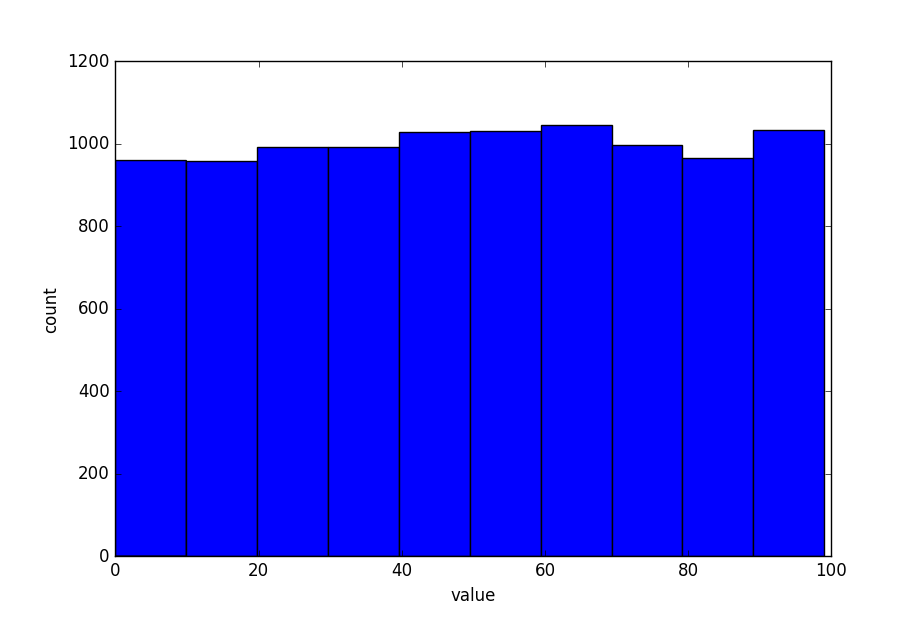
\includegraphics[width=0.4\textwidth]{./img/hist-randint.png}
\end{frame}

%%%%%%%%%%%%%%%%%%%%%%%%%%%%%%%%%%%%%%%%%%%%%%%%%%%%%%%%%%%%%%%%%%%%%%%%%%%%%%%%
\begin{frame}[fragile]
  \frametitle{Example}
  \Enlarge

  \begin{enumerate}
  \myitem  Number guessing (a game for the easily entertained):
  \end{enumerate}
  \begin{Verbatim}
import numpy as np
number = np.random.randint(10)+1
guess = input( 'Guess the number between 1 and 10:' )
while guess != number:
    guess = input( 'Nope.  Try again:' )
print( 'You did it.  Hooray.' )
  \end{Verbatim}
\end{frame}

%%%%%%%%%%%%%%%%%%%%%%%%%%%%%%%%%%%%%%%%%%%%%%%%%%%%%%%%%%%%%%%%%%%%%%%%%%%%%%%%
\begin{frame}[fragile]
  \frametitle{Example}
  \Enlarge

  \begin{enumerate}
  \myitem  Number guessing (a game for the easily entertained):
  \end{enumerate}
  \begin{Verbatim}
import numpy as np
number = np.random.randint(10)+1
guess = input( 'Guess the number between 1 and 10:' )
while int( guess ) != number:
    guess = input( 'Nope.  Try again:' )
print( 'You did it.  Hooray.' )
  \end{Verbatim}
\end{frame}

%%%%%%%%%%%%%%%%%%%%%%%%%%%%%%%%%%%%%%%%%%%%%%%%%%%%%%%%%%%%%%%%%%%%%%%%%%%%%%%%
\begin{frame}[fragile]
  \frametitle{\texttt{uniform}}
  \Enlarge

  \begin{enumerate}
  \myitem  \texttt{uniform} returns a random \texttt{float} in the range $[0,1)$.
  \end{enumerate}
  \begin{Verbatim}
np.random.uniform()      # random number, [0,1)
  \end{Verbatim}
  %\pause
  \begin{Verbatim}
np.random.uniform( size=(4,3) ) # in array
  \end{Verbatim}
  %\pause
  \begin{Verbatim}
x = np.random.uniform( size=(10000,1) )
plt.hist(x)
plt.show()
  \end{Verbatim}
  %\pause
  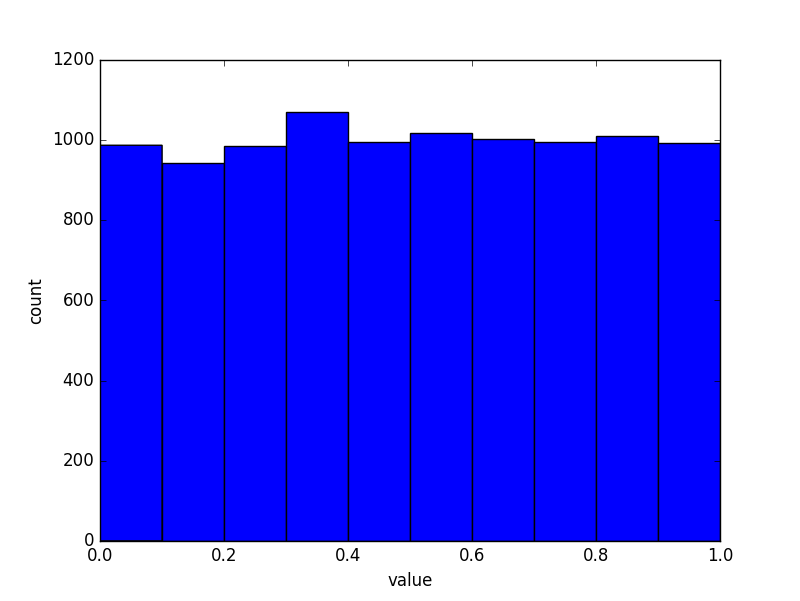
\includegraphics[width=0.4\textwidth]{./img/hist-uniform.png}
\end{frame}

%%%%%%%%%%%%%%%%%%%%%%%%%%%%%%%%%%%%%%%%%%%%%%%%%%%%%%%%%%%%%%%%%%%%%%%%%%%%%%%%
\begin{frame}[fragile]
  \frametitle{\texttt{uniform}}
  \Enlarge

  \begin{enumerate}
  \myitem  \texttt{uniform} returns a random \texttt{float} in the range $[0,1)$.
  \end{enumerate}
  \begin{Verbatim}
np.random.uniform()      # random number, [0,1)
  \end{Verbatim}
  \begin{Verbatim}
np.random.uniform( size=(4,3) ) # in array
  \end{Verbatim}
  \begin{Verbatim}
x = np.random.uniform( size=(10000,1) )
plt.hist(x,bins=100)
plt.show()
  \end{Verbatim}
  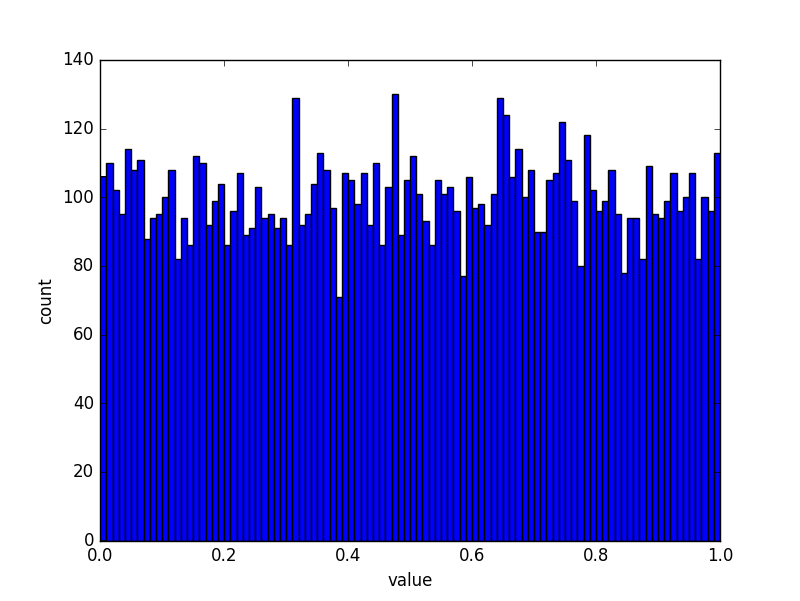
\includegraphics[width=0.4\textwidth]{./img/hist-uniform-bins.png}
\end{frame}

%%%%%%%%%%%%%%%%%%%%%%%%%%%%%%%%%%%%%%%%%%%%%%%%%%%%%%%%%%%%%%%%%%%%%%%%%%%%%%%%
\begin{frame}[fragile]
  \frametitle{\texttt{uniform}}
  \Enlarge

  \begin{enumerate}
  \myitem  \texttt{uniform} returns a random \texttt{float} in the range $[0,1)$.
  \end{enumerate}
  \begin{Verbatim}
np.random.uniform()      # random number, [0,1)
  \end{Verbatim}
  \begin{Verbatim}
np.random.uniform( size=(4,3) ) # in array
  \end{Verbatim}
  \begin{Verbatim}
x = np.random.uniform( size=(10000,1) )
plt.hist(x,bins=100)
plt.show()
  \end{Verbatim}
  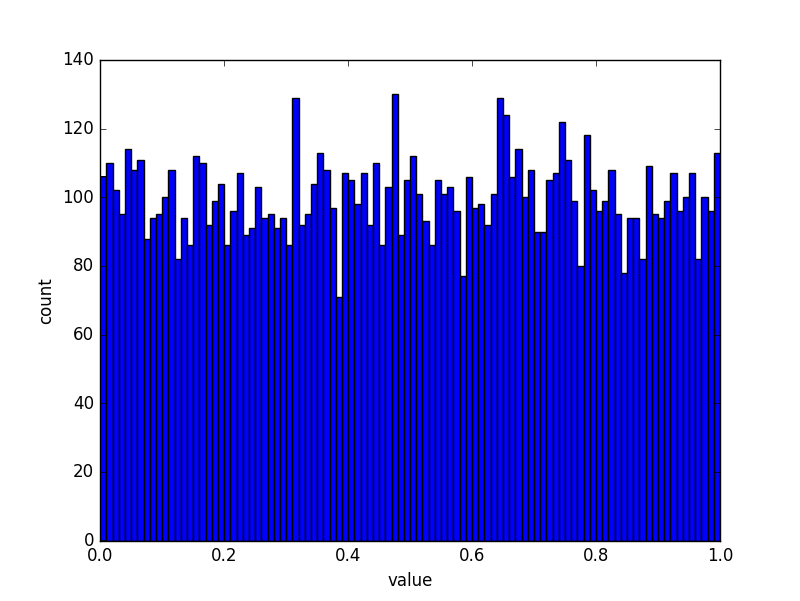
\includegraphics[width=0.4\textwidth]{./img/hist-uniform-bins.png}
\end{frame}

%%%%%%%%%%%%%%%%%%%%%%%%%%%%%%%%%%%%%%%%%%%%%%%%%%%%%%%%%%%%%%%%%%%%%%%%%%%%%%%%
\begin{frame}[fragile]
  \frametitle{\texttt{randn}}
  \Enlarge

  \begin{enumerate}
  \myitem  \texttt{randn} returns a random number selected from the \emph{normal} distribution with mean 0 and variance 1.
  \mysubitem  (Variance is the square of standard deviation.)
  \end{enumerate}
  %\pause
  \begin{Verbatim}
np.random.randn()        # random normal number
  \end{Verbatim}
  %\pause
  \begin{Verbatim}
np.random.randn() + 1.0  # mean 1.0
  \end{Verbatim}
  %\pause
  \begin{Verbatim}
(np.random.randn()) * 4  # variance 4.0
  \end{Verbatim}
\end{frame}

%%%%%%%%%%%%%%%%%%%%%%%%%%%%%%%%%%%%%%%%%%%%%%%%%%%%%%%%%%%%%%%%%%%%%%%%%%%%%%%%
\begin{frame}[fragile]
  \frametitle{\texttt{randn}}
  \Enlarge

  \begin{enumerate}
  \myitem  \texttt{randn} returns a random number selected from the \emph{normal} distribution with mean 0 and variance 1.
  \end{enumerate}
  \begin{Verbatim}
x = np.random.randn( 10000 )
plt.hist(x,bins=20)
plt.show()
  \end{Verbatim}
  %\pause
  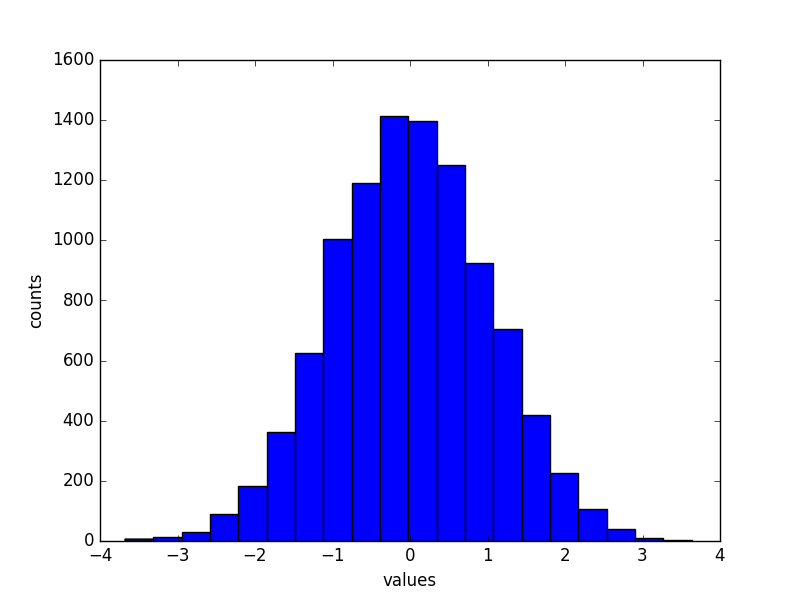
\includegraphics[width=0.4\textwidth]{./img/hist-normal.png}
\end{frame}

%%%%%%%%%%%%%%%%%%%%%%%%%%%%%%%%%%%%%%%%%%%%%%%%%%%%%%%%%%%%%%%%%%%%%%%%%%%%%%%%
\begin{frame}[fragile]
  \frametitle{\texttt{choice}}
  \Enlarge

  \begin{enumerate}
  \myitem  \texttt{choice} randomly samples a one-dimensional array (rather, the first dimension of the array).
  \end{enumerate}
  \begin{Verbatim}
x = [ 'red', 'orange', 'yellow', 'green', 'blue' ]
np.random.choice(x)      # random color
  \end{Verbatim}
\end{frame}

%%%%%%%%%%%%%%%%%%%%%%%%%%%%%%%%%%%%%%%%%%%%%%%%%%%%%%%%%%%%%%%%%%%%%%%%%%%%%%%%
\begin{frame}[fragile]
  \frametitle{\texttt{choice}}
  \Enlarge

  \begin{enumerate}
  \myitem  \texttt{choice} randomly samples a one-dimensional array but can do so \emph{without replacement}. %\pause
  \myitem  Replacement means the difference between pulling a card from a deck and putting it back before drawing again (or not). %\pause
  \end{enumerate}
  \begin{Verbatim}
x = np.arange(1,53)
c = np.random.choice( x, size=5, replace=False )
  \end{Verbatim}
  %\pause
  \begin{enumerate}
  \myitem  The foregoing code draws five cards from a deck (no repeat cards allowed).
  \end{enumerate}
\end{frame}

%%%%%%%%%%%%%%%%%%%%%%%%%%%%%%%%%%%%%%%%%%%%%%%%%%%%%%%%%%%%%%%%%%%%%%%%%%%%%%%%
\begin{frame}[fragile]
  \frametitle{\texttt{shuffle}}
  \Enlarge

  \begin{enumerate}
  \myitem  \texttt{shuffle} randomly reorders an array in place.
  \myitem  What is its return type? %\pause
  \end{enumerate}
  \begin{Verbatim}
x = np.arange(1,53)
np.random.shuffle(x)
  \end{Verbatim}
  %\pause
  \begin{enumerate}
  \myitem  The foregoing code shuffles a deck of cards.
  \end{enumerate}
\end{frame}

%%%%%%%%%%%%%%%%%%%%%%%%%%%%%%%%%%%%%%%%%%%%%%%%%%%%%%%%%%%%%%%%%%%%%%%%%%%%%%%%
\begin{frame}[fragile]
  \frametitle{Question}
  \Enlarge

  Which of the following will \emph{not} reproduce the behavior of a six-sided die in \texttt{c}?

  \begin{enumerate}[label=\Alph*]
  \item
  \begin{Verbatim}
c = np.random.randn( 6 ) + 1
  \end{Verbatim}
  \item
  \begin{Verbatim}
x = np.arange( 1,7 )
c = np.random.choice( x )
  \end{Verbatim}
  \item
  \begin{Verbatim}
c = np.random.randint( 6 )+1
  \end{Verbatim}
  \item
  \begin{Verbatim}
d = np.random.uniform( 0,6 )
c = int(d) + 1
  \end{Verbatim}
  \end{enumerate}
\end{frame}

%%%%%%%%%%%%%%%%%%%%%%%%%%%%%%%%%%%%%%%%%%%%%%%%%%%%%%%%%%%%%%%%%%%%%%%%%%%%%%%%
\begin{frame}[fragile]
  \frametitle{Question}
  \Enlarge

  Which of the following will \emph{not} reproduce the behavior of a six-sided die in \texttt{c}?

  \begin{enumerate}[label=\Alph*]
  \item
  \begin{Verbatim}
c = np.random.randn( 6 ) + 1
  \end{Verbatim}
  \correctstar
  \item
  \begin{Verbatim}
x = np.arange( 1,7 )
c = np.random.choice( x )
  \end{Verbatim}
  \item
  \begin{Verbatim}
c = np.random.randint( 6 )+1
  \end{Verbatim}
  \item
  \begin{Verbatim}
d = np.random.uniform( 0,6 )
c = int(d) + 1
  \end{Verbatim}
  \end{enumerate}
\end{frame}

%%%%%%%%%%%%%%%%%%%%%%%%%%%%%%%%%%%%%%%%%%%%%%%%%%%%%%%%%%%%%%%%%%%%%%%%%%%%%%%%
\begin{frame}[fragile]
  \frametitle{So what?}
  \Enlarge

  \begin{enumerate}
  \myitem  Our first toy example was pretty lame.  What else can we do? %\pause
  \myitem    Example:  Mad Libs
  \end{enumerate}
\end{frame}

%%%%%%%%%%%%%%%%%%%%%%%%%%%%%%%%%%%%%%%%%%%%%%%%%%%%%%%%%%%%%%%%%%%%%%%%%%%%%%%%
\begin{frame}[fragile]
  \frametitle{Mad Libs \#1}

  \begin{Verbatim}
import numpy as np

adjs = []
for line in open('adjectives.txt').readlines():
    adjs.append( line.strip() )
names = []
for line in open('names.txt').readlines():
    names.append( line.strip().split(',') )
verbs = []
for line in open('verbs.txt').readlines():
    verbs.append( line.strip().split(',') )
nouns = []
for line in open('nouns.txt').readlines():
    nouns.append( line.strip() )
# note that names and verbs have a slightly different structure
# than adj and nouns
  \end{Verbatim}
\end{frame}

%%%%%%%%%%%%%%%%%%%%%%%%%%%%%%%%%%%%%%%%%%%%%%%%%%%%%%%%%%%%%%%%%%%%%%%%%%%%%%%%
\begin{frame}[fragile]
  \frametitle{Mad Libs \#2}

  \begin{Verbatim}
adj1 = adjs[np.random.randint(len(adjs))]
noun1 = nouns[np.random.randint(len(nouns))]
name = names[np.random.randint(len(names))]
verb = verbs[np.random.randint(len(verbs))]
adj2 = adjs[np.random.randint(len(adjs))]
noun2 = nouns[np.random.randint(len(nouns))]

phrase = adj1.title() + ' ' + noun1 + ' ' + \
         name[0] + ' was so ' + adj2 + ' that ' + \
         name[1] + ' ' + verb[1] + ' a ' + \
         noun2 + '.'
  \end{Verbatim}
\end{frame}

%%%%%%%%%%%%%%%%%%%%%%%%%%%%%%%%%%%%%%%%%%%%%%%%%%%%%%%%%%%%%%%%%%%%%%%%%%%%%%%%
\begin{frame}[fragile]
  \frametitle{So what?}
  \Enlarge

  \begin{enumerate}
  \myitem  Our first toy example was pretty lame.  What else can we do?
  \myitem    Example:  Mad Libs
  \myitem    Random walk
  \end{enumerate}
\end{frame}

%%%%%%%%%%%%%%%%%%%%%%%%%%%%%%%%%%%%%%%%%%%%%%%%%%%%%%%%%%%%%%%%%%%%%%%%%%%%%%%%
\begin{frame}[fragile]
  \frametitle{Random walk \#1}

  \begin{Verbatim}
import numpy as np
import matplotlib.pyplot as plt

x = np.zeros( ( 100,1 ) )
y = np.zeros( ( 100,1 ) )
  \end{Verbatim}
\end{frame}

%%%%%%%%%%%%%%%%%%%%%%%%%%%%%%%%%%%%%%%%%%%%%%%%%%%%%%%%%%%%%%%%%%%%%%%%%%%%%%%%
\begin{frame}[fragile]
  \frametitle{Random walk \#2}

  \begin{Verbatim}
for i in range( 1,len(x) ):
    dir = np.random.randint(4)
    if dir == 0:
        x[i] = x[i-1]
        y[i] = y[i-1]+1
    if dir == 1:
        x[i] = x[i-1]+1
        y[i] = y[i-1]
    if dir == 2:
        x[i] = x[i-1]
        y[i] = y[i-1]-1
    if dir == 3:
        x[i] = x[i-1]-1
        y[i] = y[i-1]

plt.plot(x,y)
plt.show()
  \end{Verbatim}
\end{frame}

%%%%%%%%%%%%%%%%%%%%%%%%%%%%%%%%%%%%%%%%%%%%%%%%%%%%%%%%%%%%%%%%%%%%%%%%%%%%%%%%
\begin{frame}[fragile]
  \frametitle{So what?}
  \Enlarge

  \begin{enumerate}
  \myitem  Our first toy example was pretty lame.  What else can we do?
  \myitem    Example:  Mad Libs
  \myitem    Random walk
  \myitem    Think of others:  games, for instance.
  \myitem    Also, scientific applications (quantum mechanics).
  \end{enumerate}
\end{frame}

\end{document}
